% Template de LaTex para tesis del ITESM Campus Guadalajara
% Basado en el template de Word de Ra'ul Crespo Saucedo
% Basado en el sistema de guiones de Universidad Computense de Madrid
% Adaptaci'on realizada por Arturo Jafet Rodr'iguez Mu'noz
% Revision por Marco Antonio Rangel Bocardo
% Maestr'ia en Ciencias Computacionales - ITESM Campus Guadalajara
% Guadalajara, Jalisco Septiembre del 2011
% Recomiendo esta gu'ia de LaTex: http://en.wikibooks.org/wiki/LaTeX/

\documentclass[12pt,letterpaper]{report}

\usepackage{listings}
\usepackage{color}
\usepackage{amsmath,amssymb}
\usepackage{makecell}
\usepackage{etoolbox}% http://ctan.org/pkg/etoolbox



\let\Chapter\chapter
\def\chapter{\addtocontents{lol}{\protect\addvspace{10pt}}\Chapter}


\definecolor{dkgreen}{rgb}{0,0.6,0}
\definecolor{gray}{rgb}{0.5,0.5,0.5}
\definecolor{mauve}{rgb}{0.58,0,0.82}

\lstset{frame=tb,
  language=SQL,
  aboveskip=3mm,
  belowskip=3mm,
  showstringspaces=false,
  columns=flexible,
  basicstyle={\small\ttfamily},
  numbers=none,
  numberstyle=\tiny\color{gray},
  keywordstyle=\color{blue},
  commentstyle=\color{dkgreen},
  stringstyle=\color{mauve},
  breaklines=true,
  breakatwhitespace=true
  tabsize=3
}





\usepackage[spanish,activeacute]{babel}
\usepackage[T1]{fontenc}
\usepackage{graphicx}
\usepackage[letterpaper]{geometry}
\usepackage{titlesec}
\usepackage{url}
\usepackage{fancyhdr}
\usepackage{fix-cm}
\usepackage{setspace} 
\usepackage{amsmath}
\usepackage{fmtcount}
\usepackage{threeparttable}
\usepackage{float}
\usepackage[font=small,format=plain,labelfont=bf,it]{caption}
\geometry{top=2.5cm, bottom=2.5cm, left=3.0cm, right=2.5cm}
\renewcommand{\rmdefault}{cmr} % Roman
\renewcommand{\encodingdefault}{T1}
\newcommand{\subscript}[1]{\ensuremath{_{\textrm{#1}}}}
\setstretch{1.5}


%\headheight = 49pt
%\footskip = 10pt


%----------------------------------------------------------------
%
% Fichero con algunas divisiones de palabras que LaTeX no
% hace correctamente si no se le da alguna ayuda.
%
% Universidad Computense de Madrid
% http://gaia.fdi.ucm.es/projects/texis
%----------------------------------------------------------------

\hyphenation{
% a
abs-trac-to
abs-trac-tos
abs-trac-ta
abs-trac-tas
ac-tua-do-res
a-gra-de-ci-mien-tos
ana-li-za-dor
an-te-rio-res
an-te-rior-men-te
apa-rien-cia
a-pro-pia-do
a-pro-pia-dos
a-pro-pia-da
a-pro-pia-das
a-pro-ve-cha-mien-to
a-que-llo
a-que-llos
a-que-lla
a-que-llas
a-sig-na-tu-ra
a-sig-na-tu-ras
a-so-cia-da
a-so-cia-das
a-so-cia-do
a-so-cia-dos
au-to-ma-ti-za-do
% b
batch
bi-blio-gra-f\'ia
bi-blio-gr\'a-fi-cas
bien
bo-rra-dor
boo-l-ean-expr
% c
ca-be-ce-ra
call-me-thod-ins-truc-tion
cas-te-lla-no
cir-cuns-tan-cia
cir-cuns-tan-cias
co-he-ren-te
co-he-ren-tes
co-he-ren-cia
co-li-bri
co-men-ta-rio
co-mer-cia-les
co-no-ci-mien-to
cons-cien-te
con-si-de-ra-ba
con-si-de-ra-mos
con-si-de-rar-se
cons-tan-te
cons-trucci\'on
cons-tru-ye
cons-tru-ir-se
con-tro-le
co-rrec-ta-men-te
co-rres-pon-den
co-rres-pon-dien-te
co-rres-pon-dien-tes
co-ti-dia-na
co-ti-dia-no
crean
cris-ta-li-zan
cu-rri-cu-la
cu-rri-cu-lum
cu-rri-cu-lar
cu-rri-cu-la-res
% d
de-di-ca-do
de-di-ca-dos
de-di-ca-da
de-di-ca-das
de-rro-te-ro
de-rro-te-ros
de-sa-rro-llo
de-sa-rro-llos
de-sa-rro-lla-do
de-sa-rro-lla-dos
de-sa-rro-lla-da
de-sa-rro-lla-das
de-sa-rro-lla-dor
de-sa-rro-llar
des-cri-bi-re-mos
des-crip-ci\'on
des-crip-cio-nes
des-cri-to
des-pu\'es
de-ta-lla-do
de-ta-lla-dos
de-ta-lla-da
de-ta-lla-das
di-a-gra-ma
di-a-gra-mas
di-se-�os
dis-po-ner
dis-po-ni-bi-li-dad
do-cu-men-ta-da
do-cu-men-to
do-cu-men-tos
% e
edi-ta-do
e-du-ca-ti-vo
e-du-ca-ti-vos
e-du-ca-ti-va
e-du-ca-ti-vas
e-la-bo-ra-do
e-la-bo-ra-dos
e-la-bo-ra-da
e-la-bo-ra-das
es-co-llo
es-co-llos
es-tu-dia-do
es-tu-dia-dos
es-tu-dia-da
es-tu-dia-das
es-tu-dian-te
e-va-lua-cio-nes
e-va-lua-do-res
exis-ten-tes
exhaus-ti-va
ex-pe-rien-cia
ex-pe-rien-cias
% f
for-ma-li-za-do
% g
ge-ne-ra-ci\'on
ge-ne-ra-dor
ge-ne-ra-do-res
ge-ne-ran
% h
he-rra-mien-ta
he-rra-mien-tas
% i
i-dio-ma
i-dio-mas
im-pres-cin-di-ble
im-pres-cin-di-bles
in-de-xa-do
in-de-xa-dos
in-de-xa-da
in-de-xa-das
in-di-vi-dual
in-fe-ren-cia
in-fe-ren-cias
in-for-ma-ti-ca
in-gre-dien-te
in-gre-dien-tes
in-me-dia-ta-men-te
ins-ta-la-do
ins-tan-cias
% j
% k
% l
len-gua-je
li-be-ra-to-rio
li-be-ra-to-rios
li-be-ra-to-ria
li-be-ra-to-rias
li-mi-ta-do
li-te-ra-rio
li-te-ra-rios
li-te-ra-ria
li-te-ra-rias
lo-tes
% m
ma-ne-ra
ma-nual
mas-que-ra-de
ma-yor
me-mo-ria
mi-nis-te-rio
mi-nis-te-rios
mo-de-lo
mo-de-los
mo-de-la-do
mo-du-la-ri-dad
mo-vi-mien-to
% n
na-tu-ral
ni-vel
nues-tro
% o
obs-tan-te
o-rien-ta-do
o-rien-ta-dos
o-rien-ta-da
o-rien-ta-das
% p
pa-ra-le-lo
pa-ra-le-la
par-ti-cu-lar
par-ti-cu-lar-men-te
pe-da-g\'o-gi-ca
pe-da-g\'o-gi-cas
pe-da-g\'o-gi-co
pe-da-g\'o-gi-cos
pe-rio-di-ci-dad
per-so-na-je
plan-te-a-mien-to
plan-te-a-mien-tos
po-si-ci\'on
pre-fe-ren-cia
pre-fe-ren-cias
pres-cin-di-ble
pres-cin-di-bles
pri-me-ra
pro-ble-ma
pro-ble-mas
pr\'o-xi-mo
pu-bli-ca-cio-nes
pu-bli-ca-do
% q
% r
r\'a-pi-da
r\'a-pi-do
ra-zo-na-mien-to
ra-zo-na-mien-tos
re-a-li-zan-do
re-fe-ren-cia
re-fe-ren-cias
re-fe-ren-cia-da
re-fe-ren-cian
re-le-van-tes
re-pre-sen-ta-do
re-pre-sen-ta-dos
re-pre-sen-ta-da
re-pre-sen-ta-das
re-pre-sen-tar-lo
re-qui-si-to
re-qui-si-tos
res-pon-der
res-pon-sa-ble
% s
se-pa-ra-do
si-guien-do
si-guien-te
si-guien-tes
si-guie-ron
si-mi-lar
si-mi-la-res
si-tua-ci\'on
% t
tem-pe-ra-ments
te-ner
trans-fe-ren-cia
trans-fe-ren-cias
% u
u-sua-rio
Unreal-Ed
% v
va-lor
va-lo-res
va-rian-te
ver-da-de-ro
ver-da-de-ros
ver-da-de-ra
ver-da-de-ras
ver-da-de-ra-men-te
ve-ri-fi-ca
% w
% x
% y
% z
}
% Variable local para emacs, para que encuentre el fichero
% maestro de compilaci\'on
%%%
%%% Local Variables:
%%% mode: latex
%%% TeX-master: "./Tesis.tex"
%%% End:


\begin{document}
           \renewcommand{\figurename}{Figure}
           \renewcommand{\tablename}{Table}
           \renewcommand\appendixname{Appendix}

	\pagestyle{empty}
\begin{center}
\begin{center}

\includegraphics[scale=0.45]{images/escudo-itesm_small.png}
\end{center}
\vspace{15 pt}
\renewcommand{\baselinestretch}{1.0}
\Huge
%\textbf{I\hspace{1pt}n\hspace{1pt}s\hspace{1pt}t\hspace{1pt}i\hspace{1pt}t\hspace{1pt}u\hspace{1pt}t\hspace{1pt}o\hspace{1pt} \hspace{1pt}T\hspace{1pt}e\hspace{1pt}c\hspace{1pt}n\hspace{1pt}o\hspace{1pt}l\hspace{1pt}'o\hspace{1pt}g\hspace{1pt}i\hspace{1pt}c\hspace{1pt}o\hspace{1pt} \hspace{1pt}y \hspace{1pt}d\hspace{1pt}e\hspace{1pt} \hspace{1pt}E\hspace{1pt}s\hspace{1pt}t\hspace{1pt}u\hspace{1pt}d\hspace{1pt}i\hspace{1pt}o\hspace{1pt}s\\ S\hspace{1pt}u\hspace{1pt}p\hspace{1pt}e\hspace{1pt}r\hspace{1pt}i\hspace{1pt}o\hspace{1pt}r\hspace{1pt}e\hspace{1pt}s\hspace{1pt} \hspace{1pt}d\hspace{1pt}e\hspace{1pt} \hspace{1pt}M\hspace{1pt}o\hspace{1pt}n\hspace{1pt}t\hspace{1pt}e\hspace{1pt}r\hspace{1pt}r\hspace{1pt}e\hspace{1pt}y}\\
\textbf{Instituto Tecnol'ogico y de Estudios\\Superiores de Monterrey}\\
\LARGE
\textbf{Campus Guadalajara}\\
\vspace{10 pt}

\Large
\textbf{Escuela de Graduados en Ingenier'ia y\\ Arquitectura (EGIA)}\\
\vspace{20 pt}

\textbf{Maestr'ia en Ciencias de la Computaci'on}\\
\vspace{35 pt}

\Huge
\textbf{Applying Model Checking to Detect Conflicts in Rule-Based Internet Plans}\\
\vspace{50 pt}

\Large
\begin{flushleft}
\hspace{5pt}\textbf{AUTOR: \hspace{4pt}Alvaro Maza Maza}\\
\vspace{5pt}
\hspace{5pt}\textbf{ASESOR:} Dr. Gerardo Padilla Zarate \\
%\hspace{117pt}Nombre Nombre Apellido Apellido\\
%\hspace{117pt}Nombre Nombre Apellido Apellido\\
\end{flushleft}

\large
\vspace{15pt}
\textbf{Guadalajara (Jal), 01 de Octubre de 2015}
\end{center}
\clearpage

\renewcommand{\baselinestretch}{1.5}

	\pagenumbering{roman}
	%Empieza configuracion
\setstretch{1.0}
\titleformat{\chapter}{\Huge\bfseries}{\thechapter}{0 pt}{\rule{340 pt}{3 pt}\\}
\titlespacing{\chapter}{100 pt}{-25 pt}{40 pt}[10 pt]	
\pagestyle{fancy}
\fancyhead[RO,RE]{\thepage}
\fancyfoot[CO,CE]{}
%Termina configuracion

\clearpage
\thispagestyle{plain}
\par\vspace*{.35\textheight}{\centering This thesis is dedicated to my parents and family.\par}
\addcontentsline{toc}{chapter}{Dedication}

	%Empieza configuracion
\setstretch{1.0}
\titleformat{\chapter}{\Huge\bfseries}{\thechapter}{0 pt}{\rule{340 pt}{3 pt}\\}
\titlespacing{\chapter}{100 pt}{-25 pt}{40 pt}[10 pt]	
\pagestyle{fancy}
\fancyhead[RO,RE]{\thepage}
\fancyfoot[CO,CE]{}
%Termina configuracion

\chapter*{Acknowledgements}
\addcontentsline{toc}{chapter}{Acknowledgements}
\setstretch{1.5} %Regresa el interlineado a 1.5

\normalsize
\noindent I would like to express my sincere gratitude to my advisor PhD. Levi Henrique Santana de Lelis, for the continuous support and guidance during the thesis process. His valuable advice, patience and encouragement have been of great
importance for this work. \\

Besides my advisor, I would like to thank to my co$-$advisor: PhD. Santiago Franco for his insightful feedback, interest and tough questions.

To the professors of the DTI, particularly the Master Degree program with all its members, played an invaluable role in my graduate education. \\

Last, but not least, I would like to thank my Mother.
\clearpage
	%Empieza configuracion
\setstretch{1.0}
\titleformat{\chapter}{\Huge\bfseries}{\thechapter}{0 pt}{\rule{340 pt}{3 pt}\\}
\titlespacing{\chapter}{100 pt}{-25 pt}{40 pt}[10 pt]	
\pagestyle{fancy}
\fancyhead[RO,RE]{\thepage}
\fancyfoot[CO,CE]{}
%Termina configuracion

\chapter*{Abstract}
\addcontentsline{toc}{chapter}{Abstract}
\setstretch{1.5} %Regresa el interlineado a 1.5


\normalsize
\noindent
In this dissertation we present a greedy method based on the theory of supermodular optimization for selecting a subset of heuristics functions from a large set of heuristics with the objective of reducing the running time of the search algorithms. \\ 

 \cite{holte2006maximizing} showed that search can be faster if several smaller pattern databases are used instead of one large pattern database. We introduce a greedy method for selecting a subset of the most promising heuristicss from a large set of heuristics functions to guide the A* search algorithm. If the heuristics are consistent, our method selects a subset which is guaranteed to be near optimal with respect to the resulting A* search tree size. In addition to being consistent, if all heuristics have the same evaluation time, our subset is guaranteed to be near optimal with respect to the resulting A* running time. We implemented our method in Fast Downward and showed empirically that it produces heuristics which outperform the state of the art heuristics in the International Planning Competition benchmarks.

\clearpage
	%Empieza configuracion
\setstretch{1.0}
\titleformat{\chapter}{\Huge\bfseries}{\thechapter}{0 pt}{\rule{340 pt}{3 pt}\\}
\titlespacing{\chapter}{100 pt}{-25 pt}{40 pt}[10 pt]	
\pagestyle{fancy}
\fancyhead[RO,RE]{\thepage}
\fancyfoot[CO,CE]{}
%Termina configuracion

\chapter*{Resumen}
\addcontentsline{toc}{chapter}{Resumen}
\setstretch{1.5} %Regresa el interlineado a 1.5


\normalsize
\noindent
Esta tesis presenta un metodo formal para verificar planes de Internet basados en reglas, mediante Logica Temporal Lineal (LTL) y para determinar si hay conflicto entre las reglas dentro del plan. Los planes de Internet basados en reglas son formalizados y especificados utilizando nuestro modelo propuesto en Promela. \\

Escenarios actuales y futuros fueron tomados del dominio publico y utilizados para validar y explicar nuestro modelo propuesto. Todos los escenarios identificados fueron exitosamente modelados y verificados utilizando nuestro modelo en Promela y formulas LTLs introducidas como parte de nuestra tesis. \\

Los resultados obtenidos, demuestran que Model Checking es una herramienta v'alida y factible para modelar y verificar los planes de Internet basados en reglas.
\\


\clearpage
%	%Empieza configuracion
\setstretch{1.0}
\titleformat{\chapter}{\Huge\bfseries}{\thechapter}{0 pt}{\rule{340 pt}{3 pt}\\}
\titlespacing{\chapter}{100 pt}{-25 pt}{40 pt}[10 pt]	
\pagestyle{fancy}
\fancyhead[RO,RE]{\thepage}
\fancyfoot[CO,CE]{}
%Termina configuracion

\chapter*{Acknowledgments}
\addcontentsline{toc}{chapter}{Acknowledgments}
\setstretch{1.5} %Regresa el interlineado a 1.5

\normalsize
\noindent TBD
\clearpage%

	\renewcommand{\baselinestretch}{1}
\titleformat{\chapter}{\Huge\bfseries}{\thechapter}{0 pt}{\rule{340 pt}{3 pt}\\}
\titlespacing{\chapter}{100 pt}{-25 pt}{40 pt}[10 pt]	
\renewcommand{\baselinestretch}{1.5}
\renewcommand{\contentsname}{Table of Contents} 
\tableofcontents
\renewcommand{\baselinestretch}{1.5}
	\renewcommand{\baselinestretch}{1}
\titleformat{\chapter}{\Huge\bfseries}{\thechapter}{0 pt}{\rule{340 pt}{3 pt}\\}
\titlespacing{\chapter}{100 pt}{-49 pt}{40 pt}[10 pt]	
\renewcommand{\listtablename}{List of Tables} 
\listoftables
\addcontentsline{toc}{chapter}{List of Tables}
\renewcommand{\baselinestretch}{1.5}

	\renewcommand{\listfigurename}{List of Figures} 
\renewcommand{\baselinestretch}{1}
\titleformat{\chapter}{\Huge\bfseries}{\thechapter}{0 pt}{\rule{340 pt}{3 pt}\\}
\titlespacing{\chapter}{100 pt}{-49 pt}{40 pt}[10 pt]	
\listoffigures
\addcontentsline{toc}{chapter}{List of Figures}
\renewcommand{\baselinestretch}{1.5}

	\renewcommand{\baselinestretch}{1.0}
\titleformat{\chapter}{\Huge\bfseries}{\thechapter}{0 pt}{\rule{340 pt}{3 pt}\\}
\titlespacing{\chapter}{100 pt}{-49 pt}{40 pt}[10 pt]	
\lstlistoflistings
\addcontentsline{toc}{chapter}{Listings}
\renewcommand{\baselinestretch}{1.5}


	\pagenumbering{arabic}
	%Empieza configuracion de capitulo
\setstretch{1.0}
\titleformat{\chapter}[block]{\Large\bfseries}{CHAPTER \Huge\thechapter\vspace{25 pt}}{0 pt}{\\\fontsize{26}{36}\selectfont}
\titlespacing{\chapter}{0 pt}{30 pt}{50 pt}[0 pt]
\titleformat{\section}{\Large\bfseries}{\thesection}{0 pt}{\hspace{30 pt}}
\titleformat{\subsection}{\large\bfseries}{\thesubsection}{0 pt}{\hspace{30 pt}}
\pagestyle{fancy}
\renewcommand{\chaptername}{CHAPTER}
\fancyhead[LO,LE]{\footnotesize\textit{\leftmark}}
\fancyhead[RO,RE]{\thepage}
\fancyfoot[CO,CE]{}
%Termina configuracion de capitulo
\chapter{Introduction} %Cambia Introducci'on al nombre de tu capitulo
\setstretch{1.5} %Regresa el interlineado a 1.5
\normalsize
\section{Background}
\vspace{30 pt}
\noindent
Internet is a collection of inter-connected private networks. These networks are operated by many Internet service providers (ISPs) or Network Operators in the world. How these networks interact with each other has strongly changed over the past years.\\

Just a decade ago, Internet users were just starting to use high-speed broadband access. By that time, there were only 569 million Internet users and we could download a song in around 10 minutes. Now, things changed and we are over 2.27 billion Internet users in the world and Real-time entertainment is, by far, the largest category of Internet traffic. \\

In order to sustain profitable business models, network operators are now looking at new ways of pricing models, beyond the standard expectation of volume-based plans \cite{Sen2013}. \\

Particularly, mobile operators have realized that they need to offer a number of flexible and smartly designed data packages, aligned to the budgets of different customer segments and target groups. As an example, several mobile operators are now offering free access to certain applications such as Facebook or WhatsApp. \\

\section{Problem Statement and Motivation}
\noindent
During the development of Broadband Plans, Network Operators specify several rules to make each plan. A rule generally defines an action to either allow or block certain applications. More complex rules, add additional constraints, such as a predefined bandwidth or a limited amount of bytes to be consumed over a period of time. \\

While a Broadband Plan is composed of one or more of these rules, they are usually designed individually and developed independently to offer new plan options to customers. When rules are added to a particular plan, an unexpected conflict may rise with the existing rules of the plan. For instance, when a new rule, such as \textit{Unlimited Facebook}, which allows unlimited access to Facebook traffic, is added to a plan already including a rule to limit up to 1GB of monthly usage, a conflict happens in the case when Facebook traffic is generated and these two rules are configured. The reason is that these two rules can be applied to the Facebook traffic. \\
	
Such conflicts are best resolved as early as possible -- ideally before the implementation of those rules. This work is motivated by the desire to prove if Model Checking can be used to detect such those conflicts. \\

Nowadays, Internet plans are evolving quickly. In fact, network operators are moving from unlimited or volume-based models to value-added data offerings \cite{Sen2013,Kimbler2012}. Consequently, it is reasonable to predict that their offer of plans will soon include a non-small number of rules, including conditions such as its current location, device, current time of the day, etc. Subscribers may even have the option to select the rules to make their own plan. \\

In order for us to use Model Checking to detect conflicts between rules within a plan, we first need to design a generic model to specify the different plans. Afterwards, we can use a formal verification language to exhaustively and automatically check whether the model meets the plan specification and to detect conflicts between the rules in the plan. 

\section{Aim and Objectives}
\subsection{Aim}
\noindent
Explore the use of formal methods to identify conflicts between rules, within an Internet Plan. A popular technique known as model-checking has been used in many other domains. Our aim is to apply model checking to verify the model of rule-based Internet Plans and identify conflicts.  

\subsection{Objectives}
\noindent
\begin{itemize}
\item Create an abstract model to specify the rule-based Internet Plans.
 
\item Implement algorithms to complement the model-checking verification.

\item Define real and future use-cases scenarios based on Internet Plans offered in the public domain. 

\item Exhaustively and automatically check whether the model meets the specification of the plan.

\item Detect if there is any conflict between two or more rules within the rule-based Internet plan. 

\end{itemize}

\section{Scope, Limitations, and Delimitations}
\noindent
The model described in this Thesis was based on the fact that Internet plans, and Network Policies, have been commonly expressed in the form of rules and actions. Network specifications evolved from Network Policy languages, found in \cite{rfc1102,Sloman1999,Stone2001}, to the well-known and currently widely-used 3GPP Architecture, found in \cite{Albaladejo2008,Grgic2013}. \\

Network operators using 3GPP-based technologies, requires to specify their plans in the form of rules and actions. 3GPP defines a 5-tuple set of classifiers: source IP address, destination IP address, source port number, destination port number, and protocol ID of the protocol above IP to identify a flow. However, many Network Operators are also extending them, to other classifications such as protocol/application, location and device. \\

A verification modeling language will be used to specify a number of current and future use-cases scenarios found in the public domain.  Those use-cases will be verified against their expected properties expressed as Linear Temporal Logic (LTL) formulas. \\

The outcome of this Thesis is to prove that Model Checking is a feasible approach to specify and verify rule-based Internet plans; bearing in mind that plans with many rules would require much more CPU resources. Other methods or approaches to specify and verify such those plans are out-of-scope of this research.

\section{Justification}
\noindent
World$'$s population is expected to exceed 7.6 billion early in 2020, up from the current 7.2 billion; while the number of internet-connected devices is expected to double in 5 years, from 25 billion, now in 2015, to 50 billion by 2020 \cite{Evans2011}.  \\

With this proliferation of Internet-connected devices, essentially the number of Internet-connected devices in the world has grown faster than the number of people in the World, network operators are trying to differentiate themselves by offering new ways of pricing models, beyond the usual vectors of volume and bandwidth.\\

In most industries, customers have a choice in selecting the expected quality, which is usually tied to a well-known categorization. In the airlines industry, economy or business tickets can be bought. In the Hotel industry, the quality is dictated by the number of stars. \\

Particularly in the world of fast-food restaurants, we have seen an evolution in the last 5 years. At the very beginning, the meals were fixed and simple. Now the meal options got more varied and, in some fast-food chains, it is even possible to choose all the \textit{features} in your meal: which kind of bread, which kind of ham, which dressing, and so on \cite{Cheboldaeff2011}. \\

On the other hand, in the world of Retail, we see examples of a new micro payment economy. Rather than long term commitments, people are making compulsives small purchases. As an example we can see people renting a house for weekly basis, or hourly renting a car, or even purchasing certain songs and not entire albums. \\

In the world of broadband data, network operators are also rethinking the notion of  the long term contracts and fixed tiered plans. Network Operators are basically moving from unlimited or volume-based models to value-added data offerings to basically offer price transparency and access to certain applications for specified amounts of time, at affordable rates \cite{Kimbler2012}. For example, Vox Telecom, a DSL provider in South Africa, partnered with a local retailer around the launch of the game ``Call of Duty: Black Ops II'' to provide 40GB of ``gamer optimized'' ADSL Bandwidth to customers who redeemed a voucher included with the purchase of the game \cite{Sandvine2014}. Similarly, China Mobile currently offers ``Lite Data Service Plans'' at reduced prices, where heavy-data-usage applications, such as Peer-To-Peer applications, are blocked, in order to rationalize the use of the data plans \cite{ChinaMobile2015}. \\

Given that Network Operators are moving to value-added Internet plans, the spectrum of possible combinations of rules to form plans is huge. Consequently, Network Operators will require tools to validate the rules within a plan, and most importantly, an automated system that verifies the rule-based plans against its specification and that finds any possible conflict among the rules. \\

In that sense, Model Checking can be used to exhaustively and automatically establish whether a given rule-based Internet Plan, satisfies a predefined set of properties (formal specification) and determine whether or not there is a conflict within the rules. \\

\section{Hypothesis}
\noindent
This thesis will intend to prove the hypotheses listed below:
\begin{itemize}
\item \textbf{H1:} Rule-based Internet plans can be abstracted and specified in  a verification modeling language. 

\item \textbf{H2:} Model Checking can be used to verify whether the model meets the specification of the plan and to detect conflicts between the rules within the plans. 
\end{itemize}

\section{Contribution of the Thesis}
\noindent
The main contributions of this Thesis are:
\begin{itemize}
\item Provide a framework to specify rule-based Internet plans via a verification modeling language. This model will let specify the rules-based Internet Plans unambiguously.  
\item Provide real and future use-cases scenarios based on Internet Plans offered in the public domain. These scenarios will let us verify our proposed model with their properties. 
\item Provide a set of LTL formulas to exhaustively and automatically verify rule-based Internet plans. These LTL formulas will let us verify the identified scenarios and any other possible plan specified with our proposed model.   
\item Prove that Model Checking is a powerful approach to detect conflicts between the rules within Internet plans. 
\end{itemize}

\section{Organization of the Thesis}
\noindent
The Thesis is organized as follows: 
\begin{enumerate}
\item In Chapter 1, the introduction to the thesis is provided which also includes our motivation and defines its scope. 
\item In Chapter 2, we review the State of the Art.
\item In Chapter 3, we introduce our model to specify the Rule-based Internet Plans, and the LTL to be used to verify them. 
\item In Chapter 4, we introduce MexCom, a not real Mexican Mobile Operator company offering use-cases we found in the Public Domain. 
\item In Chapter 5, we validate the use-cases described in the previous chapter with the model studied in chapter 3. The results are analyzed and discussed at the end of the chapter.
\item We conclude in Chapter 6 by discussing further improvements and future work.
\end{enumerate}

In the next chapter, the evolution of Internet Plans is reviewed and Model Checking is explained and discussed as a widely-used approach in many other domains. \\

\clearpage
	%Empieza configuracion de capitulo
\setstretch{1.0}
\titleformat{\chapter}[block]{\Large\bfseries}{CHAPTER \Huge\thechapter\vspace{25 pt}}{0 pt}{\\\fontsize{26}{36}\selectfont}
\titlespacing{\chapter}{0 pt}{30 pt}{50 pt}[0 pt]
\titleformat{\section}{\Large\bfseries}{\thesection}{0 pt}{\hspace{30 pt}}
\titleformat{\subsection}{\large\bfseries}{\thesubsection}{0 pt}{\hspace{30 pt}}
\pagestyle{fancy}
\renewcommand{\chaptername}{CHAPTER}
\fancyhead[LO,LE]{\footnotesize\textit{\leftmark}}
\fancyhead[RO,RE]{\thepage}
\fancyfoot[CO,CE]{}
%Termina configuracion de capitulo

\chapter{Literature Review} 
\setstretch{1.5} %Regresa el interlineado a 1.5

\normalsize

\section{Mobile Broadband services}
\noindent

\subsection{Evolution}
\noindent
There seems to be a consensus on how mobile broadband services have evolved and, more importantly, in which direction they go. In 2012, Kimbler and Taylor characterized the evolution of strategies for mobile broadband data services in three phases as follows \cite{Kimbler2012}:
  \begin{itemize}
      \item Phase One: Unlimited data plans.
      \item Phase Two: Volume-based charging.
      \item Phase Three: Value-added mobile broadband services.
    \end{itemize} \bigskip

Ezziane was not wrong when in 2005 predicted that the traditional flat rate will no longer be valid. Instead,  accounting and billing for emerging 3G services will be content-based and usage-based \cite{Ezziane2005}. \\

In 2013, Sen et al, introduced the term Smart Data Pricing (SPD), described as a broad set of ideas and principles that go beyond the traditional at-rate or byte-counting models. Such SDP models can include any of the following mechanisms: Time-based, location-based, application-based, quota-aware content distribution \cite{Sen2013}. \\

\begin{figure}[H]
\centering
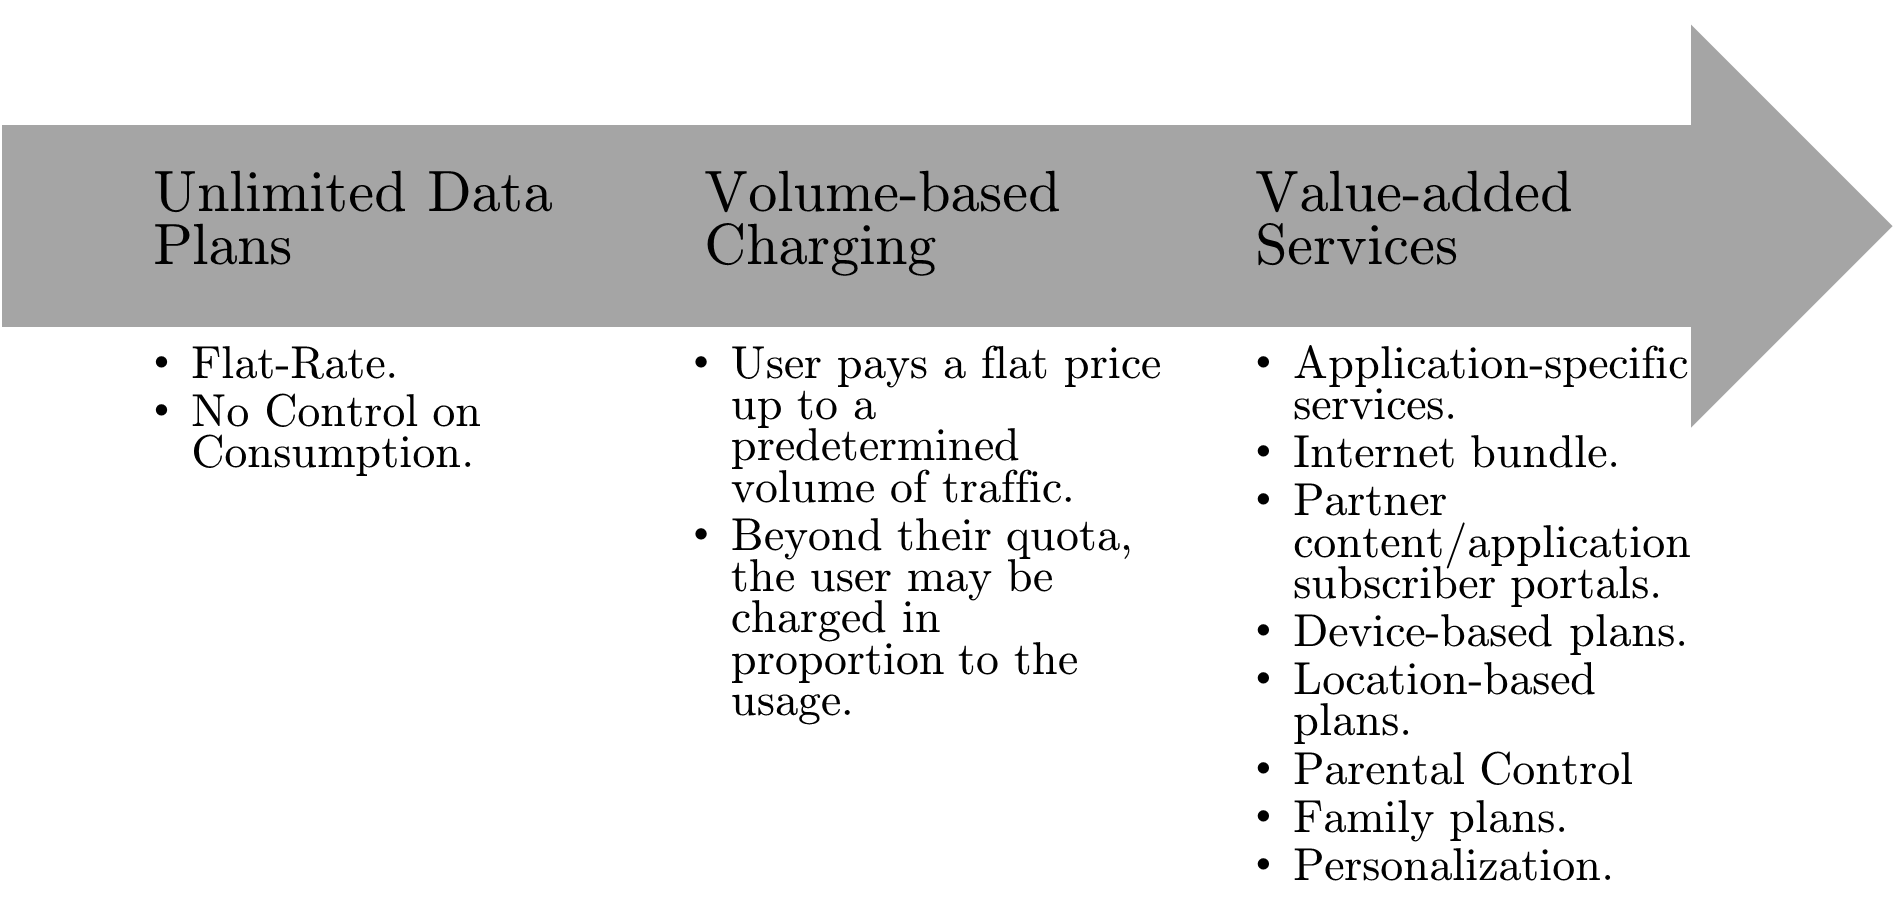
\includegraphics[width=1.00\textwidth]{image/Evolution}
\caption{Evolution of the Mobile Broadband services \cite{Kimbler2012}}
\end{figure}

Later in 2013, Hart and Brown defined similar services to be enabled on an LTE network: Fair usage, Time of Day, Parental Control, Shared Data Plans, Turbo Boost, Bundling of Popular Services (e.g. Twitter, Facebook, etc.) and HD Voice and Video \cite{Hart2013}.\\

Similarly to the authors mentioned above, telecommunication companies have also published their research regarding this topic. For example in 2012, Elitecore Technologies listed a number of emerging use cases, such as: turbo boost, family plans, application-based \& device-based plans, service personalization, etc \cite{Elitecore2012}. While Sandvine, which offers solutions to communication service providers (CSPs), talks about: Application-based service tiers and bolt-ons, roaming packages, shared data plans, sponsored connectivity and third-party bundles \cite{Sandvine2014_2}. Nowadays, Alcatel Lucent and Allot Communications, other telecommunication companies, are also offering solutions about application-based charging, turbo boost and Parental Control \cite{Alcatel2014,Allot2014}. \\

It is clear that network operators have already started to create value added data services and specialized packages that can be sold on top of or instead of the traditional tiered volume-based data packages. This approach is allowing operators to create incremental data revenues and effectively monetize their data traffic in an smarter way \cite{Kimbler2012}.

%Agregar principales problemas perdidas, susbcribers de bajos recursos, etc.%
\subsection{Examples of value-added services}
\noindent
The table \ref{usecases} below, provides an overview of some of the most common volume and value added data services available today. The real advantage of value-based data plans is that they are designed to meet the wants and needs of the end-users and customers \cite{Elitecore2012}.
\begin{table}[H]
\begin{center}
\scalebox{0.8}{	
\begin{tabular}{| l || p{6.2cm} | p{8.2cm} |}
\hline
\textbf{Pricing Policy} & \textbf{Description} & \textbf{Example of Global Telco's} \\
 \hline \hline
\emph{Access Network} & Policy based on the access network. e.g. 2G, 3G, 4G, WiFi, WiMax. & AT\&T, Verizon, T-Mobile (USA), Movistar (Colombia), MTS(Russia), Aircel, Celcom, Singtel.   \\ \hline
\emph{Tiered Plans} & Different Quota-based plans with FUP and overage. & AT\&T, Verizon, T-Mobile (USA), Celcom, Movistar (Colombia), Singtel, Aircel, Vodafone (India).    \\ \hline
 \emph{Device-based plans} & Plans based on the accessed device. e.g. iPad, iPhone, Smart TV, Laptop & AT\&T, Verizon, T-Mobile (USA),Celcom, Movistar (Colombia), MTS(Russia), Aircel, Singtel. \\ \hline
 \emph{Parner-based plans} & Partner-based plans enable operators offer content at subsidized rate. & AT\&T, Verizon, T-Mobile (USA), Maxis, Celcom, SingTel, Aircel, Vodafone (India). \\ \hline
 \emph{Parner-based plans} & Partner-based plans enable operators offer content at subsidized rate. & AT\&T, Verizon, T-Mobile (USA), Maxis, Celcom, SingTel, Aircel, Vodafone (India). \\ \hline
 \emph{Time-based plans} & Time of day, hourly plans, Seasonal plans. & AT\&T, Movistar (Colombia), MTS (Russia), Maxis, Celcom. \\ \hline
 \emph{Service Personalization} & Subscribers can self select from webselfcare. & AT\&T, Verizon, T-Mobile (USA), Movistar (Colombia), MTS (Russia), Maxis, SingTel, Aircel. \\ \hline
 \emph{Parental Control} & Quota management or Application control for child account. & AT\&T, Verizon, Verizon, Maxis.\\ \hline
 \emph{Application/Service} & Application specific charges, e.g. Social networking bundles, emails, etc. & Movistar (Colombia), Maxis, Celcom, SingTel.\\ \hline
 \emph{Family-based Plans} & Data plans with common data pool and sharing & T-Mobile (USA).\\ \hline
\end{tabular}}
\end{center}
\caption{Key use-cases listed by \emph{Elitecore Technologies} in \cite{Elitecore2012}. }
\label{usecases}
\end{table}

\section{Broadband communications technologies}
\noindent
Conflicts among policy rules within a particular plan are the core focus of this thesis. However, the interaction between technologies and the offered services should be well understood. Essentially, all plans are built on top of technologies.\\ 

In order to offer value-added services, network operators need powerful tools to inspect, measure and analyze data traffic in more sophisticated ways that they have done in the past. \\

Several leading vendors including Comverse, Sandvine, Openet, Allot, Huawei and Amdocs have seized this market opportunity and offer comprehensive data traffic management solutions that combine:
  \begin{itemize}
      \item Policy Control (PCRF/PCEF).
      \item Deep Packet Inspection (DPI).
      \item On-line Data Rating and Charging.
	  \item Bandwidth Control and QoS Management.
      \item Content Filtering, Caching and Compression.
	  \item Business Intelligence and Analytics.
    \end{itemize} \bigskip

In the past, many operators used technologies like policy management or DPI to solve specific problems with network congestion, assure fair usage and satisfy regulatory requirements, but they rarely used them to generate new revenue streams \cite{Kimbler2012}.\\	

Operators are showing early interest in using a combination of DPI and policy management to offer value-added services on top of their existing basic packages.

\section{Model Checking}
\noindent
A model can be seen as a simplification of reality. We build models to better understand things, and most importantly, to describe part of a system from a particular perspective. Additionally, a model let us describe unambiguously the system itself or its properties. In this section, we focus on modeling languages and how can we prove or disprove the correctness of it with regards to a specification. \\

A modeling language is any artificial language that can be used to express information or knowledge or systems in a structure that is defined by a consistent set of rules. One of the key benefits of using a modeling language, is that it will let us verify it formally against a given specification. \\ 

Formal verification is the process of applying a manual or automatic formal technique for establishing whether a given system satisfies a given property or behaves in accordance to some abstract description (formal specification) of the system. This verification is done by software tools as model checkers. A model checker thoroughly explores the state space to decide whether the system satisfies the set of properties. \\

Figure \ref{modelChecking} below, illustrates the overall process of Model Checking \cite{Chan1998}. In a first step, which is called modeling, the system description is converted into the system model. The requirements have to be manually formalized because they are mostly given in natural language. The result of this formalization is the formal specification given as formulas in a temporal logic such as LTL (Linear Temporal Logic). \\

As shown below, the model and the specification are inputs given to the model checker. The model checker uses an exhaustive search over all reachable states of the model to check whether the model satisfies the formula. In the end, it returns a result. The result may be that the model satisfies the formula or that the model does not satisfy the formula.  \\

\begin{figure}[H]
\centering
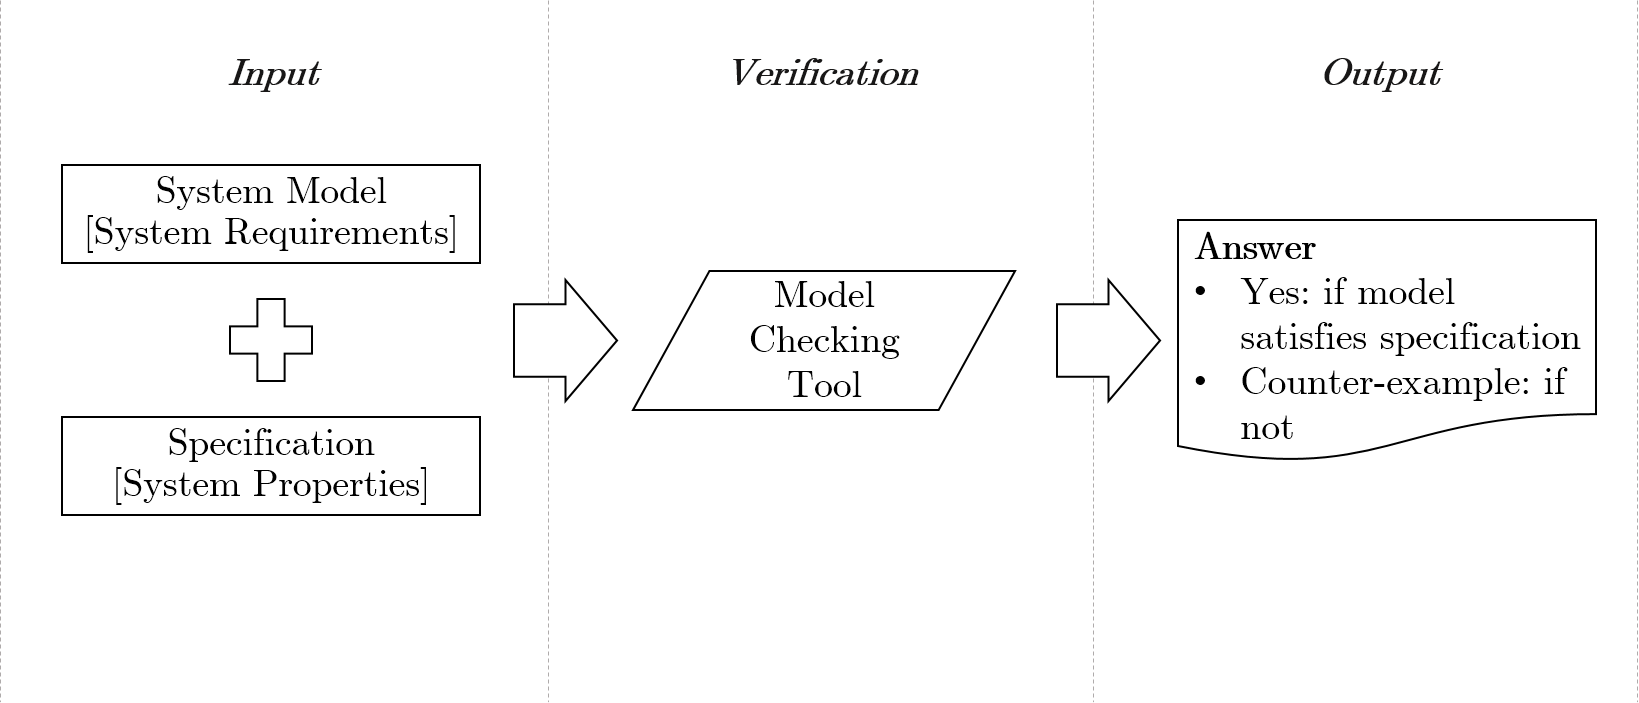
\includegraphics[width=0.95\textwidth]{image/ModelChecking}
\caption{Model checking process}
\label{modelChecking}
\end{figure}

\bigskip

\subsection{Spin Model Checker and PROMELA}
\noindent
Spin and most of its predecessors are implementations of standard automata-based reachability analyzers, with primary emphasis on performance. It provides an efficient implementation of a classic reachability analyzer with a firm and well-understood theory for LTL model checking \cite{holzmann2000spin} - or also known as the VardiWolper framework for automata-theoretic verification \cite{Vardi1986}. It supports the use of LTL (linear temporal logic) for the specification of correctness properties.\\

Spin accepts specifications written in a meta-language named Promela (Process Meta Language). Promela is a verification modeling language introduced by Gerard J. Holzmann. The language allows for the dynamic creation of concurrent processes to model, for example, concurrent or distributed systems. The three main types of objects that can be manipulated are: 
  \begin{itemize}
      \item processes,
      \item channels, and
      \item variables. 
    \end{itemize} \bigskip

Spin represents the system as a finite state machine. It visits each reachable state explicitly using Nested DFS and using partial order reduction. If a property is specified in LTL, Spin will first convert the LTL formula into an equivalent never claim, using the procedure outlined in \cite{Gerth1995}. Formally, the never claim specifies a Buchi automaton (a specific type of omega automaton) and the acceptance conditions from this automaton are evaluated on the global systems execution graph \cite{holzmann2000spin}. The efficiency of the Spin system comes from its on-the-fly procedure for performing this check that requires only small amounts of memory to be consumed for each state that is reached. The details of this so-called nested depth-first search algorithm are documented in \cite{Holzmann1996}. 

\subsubsection{Data Types}
\noindent
In Promela, there are seven predefined integer data types: bit, bool, byte, pid, short, int, and unsigned . There are also constructors for user-defined data types, and there is a separate predefined data type for message passing channels. Variables of type bit and bool are stored in a single bit of memory, which means that they can hold only binary, or boolean values.  \\

Typedef declarations can be used to introduce user-defined data types. User-defined data types can use any predefined integer data types. 

\subsection{Linear Temporal Logic - LTL}
\noindent
Spin, as any other model checker, needs a number of system properties to verify the System Model (expressed in Promela). Without the system properties, the model checker cannot really tell whether or not the System Model is correct. In Promela, Linear Temporal Logic is used for specifying the correctness of requirements. \\

Linear temporal logic (LTL) is a modal temporal logic with modalities referring to time. In LTL, one can encode formulas about the future of paths, e.g. a condition will eventually be true, a condition will be true until another fact becomes true, etc. It is a fragment of the more complex CTL*, which additionally allows branching time and quantifiers. 
\clearpage
LTL is built up from a finite set of propositional variables, logical operators (i.e. $\neg$, $\land$, $\lor$, $\implies$, $\iff$, \emph{true} and \emph{false}), and four additional temporal modal operators.

\begin{table}[H]
\begin{center}
\scalebox{0.8}{	
\begin{tabular}{| l || l | l |}
\hline
\textbf{LTL Formula} & \textbf{Description} & \textbf{Semantics Meaning} \\
 \hline \hline
$\square$ $\phi$ & Always & $\phi$ is satisfied at every state. \\ \hline
$\lozenge$ $\phi$ & Eventually & $\phi$ is satisfied at some state. \\ \hline
$\psi$ U $\phi$ & Until & $\psi$ has to hold at least until $\phi$, which holds at the current or a future position. \\ \hline
X $\phi$ & Next & $\phi$ has to hold at the next state. \\ \hline
\end{tabular}}
\end{center}
\caption{Semantics for the temporal operators}
\label{tem_operators}
\end{table}

An important taxonomy of properties, as given below, is found in many books and papers \cite{Schneider2004}. Safety and liveness properties described below, are of our particular interest; as most of our specifications are safety and liveness properties. \\

\emph{Safety properties} state that for all computations of the system, and for all instances of time, some property will invariantly hold. Colloquially, Safety properties assert that something \textquotedblleft bad\textquotedblright never happens. For example, a safety property could be defined as: \emph{Facebook traffic will never be blocked}. \\

\emph{Liveness properties} state that some desired state of the system can eventually be reached. Colloquially, a Liveness property makes sure that something \textquotedblleft good\textquotedblright  eventually happens. An example of a liveness property could be: \emph{If any other traffic is generated, it will eventually be blocked}. \\

\emph{Persistence properties} are related to the stabilization of certain properties. In general, a persistence property describes that for all possible computations, there is a point of time when a certain property will always hold afterwards. For example: there is a point where rule A is always enabled.\\

\emph{Fairness properties} state that some property will hold infinitely often. For example: No process is ignored infinitely often by an O.S. 
\section{Related Work}
\noindent
Model checking, or property checking, has been widely used in many other domains to exhaustively and automatically check whether a given model meets a given specification. Our primary interest is the use of Promela as the Model Checking tool to detect conflicts, via LTL formulas, in rules-based plans. \\

One of the main contributions for this Thesis is the research done by Zhiping Duan in 2003 \cite{Duan2003}. In his work, he provides an approach to automatically detect feature interactions (i.e. conflicts) in telecommunications systems, which are not essentially rules-based. Even though, Duan uses LTL and FOL (First-Order-Logic) to prove their systems, he proposed an implementation of a FOL prover in $\lambda$Prolog. We think it is more intuitively to use Promela for our particular domain, as Promela is a verification modeling language which directly allows LTL formulas for its verification. \\

In 2007, Antoniou, et al, integrate several aspects of policy specification languages (i.e. rule-based reasoning), in a common framework. One key contribution from his research to our Thesis, is the use of priorities to resolve conflict among rules. In his research, the implementation of a conflict checker was not addressed. \\

Between 2010 and 2011, several requirements frameworks for business process compliance management have been proposed. In \cite{Abramowicz2010,Hantry2011}, the authors formulate requirements for compliance rules. The requirements address the issues of lifetime compliance. The focus is also on the requirements to languages expressing compliance rules, on the rules priority, and on validation of process models against rules during design time and runtime. \\

In 2012, Gawanmeh, et al, proposed a novel algorithm for detecting conflicts in firewall rules \cite{Gawanmeh2012}. Even though his novel approach, using domain restriction, is interesting; its proposed algorithm doesn't consider rules with multiple types of conditions. \\

The review of the related work above, illustrates that the problem of conflicts among rules exists in different domains and, more importantly, Model-Checking is a proven approach for detecting the conflicts efficiently. In this Thesis, we will use Promela to detect conflicts in a particular area of telecommunications: rule-based Internet Plans. \\ 

\section{Summary of the chapter}
\noindent
The literature review is summarized below:
   \begin{itemize}
      \item Network Operators are basically moving from unlimited or volume-based models to value-added data offerings. These value-added services comprise a number of custom rules to form a Plan. 
      \item Because all of these services are built on top of technologies, there are a number of technical, commercial, regulatory or integration impacts, that needs to be considered when designing these value-added services. 
      \item Model Checking can perfectly be used to exhaustively and automatically verify whether a model meets a given specification. In our case the rule-based plans will be modeled using Promela and the specification will be defined in LTL. 
	  \item The problem of conflicts among rules has been studied in many other domains and, more importantly, Model-Checking is a proven approach for detecting the conflicts efficiently.
	  \item In this Thesis, Promela will be used to detect conflicts in a particular area of telecommunications: rule-based Plans.
    \end{itemize} \bigskip

In the next chapter, we will introduce the model proposed for specifying the rule-based plans and will expand on the LTL properties to verify the proposed model. \\

\clearpage
	%Empieza configuracion de capitulo
\setstretch{1.0}
\titleformat{\chapter}[block]{\Large\bfseries}{CHAPTER \Huge\thechapter\vspace{25 pt}}{0 pt}{\\\fontsize{26}{36}\selectfont}
\titlespacing{\chapter}{0 pt}{30 pt}{50 pt}[0 pt]
\titleformat{\section}{\Large\bfseries}{\thesection}{0 pt}{\hspace{30 pt}}
\titleformat{\subsection}{\large\bfseries}{\thesubsection}{0 pt}{\hspace{30 pt}}
\pagestyle{fancy}
\fancyhead[LO,LE]{\footnotesize\textit{\leftmark}}
\fancyhead[RO,RE]{\thepage}
\fancyfoot[CO,CE]{}
%Termina configuracion de capitulo

\chapter{Greedy Random Heuristic Selection (GRHS)} %Cambia al nombre de tu capitulo
\setstretch{1.5} %Regresa el interlineado a 1.5

\lstset{
language=Promela,
numbers=left,
numberstyle=\small,
frame=tb,
columns=fullflexible,
showstringspaces=false,
framexleftmargin=15pt
}

\normalsize
\noindent
The purpose of this section is to introduce the meta$-$reasoning proposed for specifying ...  
\section{--}
\subsection{Overview}
\noindent


In the next chapter, ....

\clearpage
           %Empieza configuracion de capitulo
\setstretch{1.0}
\titleformat{\chapter}[block]{\Large\bfseries}{CHAPTER \Huge\thechapter\vspace{25 pt}}{0 pt}{\\\fontsize{26}{36}\selectfont}
\titlespacing{\chapter}{0 pt}{30 pt}{50 pt}[0 pt]
\titleformat{\section}{\Large\bfseries}{\thesection}{0 pt}{\hspace{30 pt}}
\titleformat{\subsection}{\large\bfseries}{\thesubsection}{0 pt}{\hspace{30 pt}}
\pagestyle{fancy}
\fancyhead[LO,LE]{\footnotesize\emph{\leftmark}}
\fancyhead[RO,RE]{\thepage}
\fancyfoot[CO,CE]{}
\newcommand{\tabitem}{~~\llap{\textbullet}~~}
%Termina configuracion de capitulo

\chapter{Case Study: MexCom Use Cases} %Cambia al nombre de tu capitulo
\setstretch{1.5} %Regresa el interlineado a 1.5

\normalsize
\noindent
In this chapter, we present the rule-based plans, which will be verified using the Promela Model described in the previous chapter. \\

We begin this chapter by introducing ``MexCom'', a not real company we created to illustrate the number of use-cases described below. We build the use-cases, based on the rules-based plans found in the Public Domain. We also considered some not-yet-existing rules; which, based on the literature review, are quite reasonable to predict. \\

In the next chapter, MexCom plans will be modeled using our proposed Promela Model and verified through the LTL formulas previously studied. \\

\section{MexCom Overview}
\noindent
MexCom is a new Mobile Network Operator, which is eager to start operations in Mexico soon. MexCom will target low-income subscribers, who cannot afford an unlimited mobile plan. \\

The next sections describe the evolution of the service plans MexCom will offer to gain market share. It is important to mention that a plan will consist of one or more rules described below.   

\section{Core Rules}
\noindent
MexCom wants to start operations in Mexico by offering an initial set of monthly limited usage rules, which are listed below in table \ref{LUP_initial} \\

\begin{table}[H]
\begin{center}
\scalebox{0.8}{	
\begin{tabular}{| l || r | r |}
\hline
\textbf{Core Rule ID} & \textbf{Capacity} & \textbf{Monthly Cost (MXN)} \\
 \hline \hline
\emph{CORE01} & 100MB & {\$}75.00   \\ \hline
\emph{CORE02} & 200MB & {\$}100.00   \\ \hline
\emph{CORE03} & 400MB & {\$}150.00   \\ \hline
\emph{CORE04} & 1GB & {\$}350.00   \\ \hline
\emph{CORE05} & 2GB & {\$}600.00   \\ \hline
\end{tabular}}
\end{center}
\caption{Core Limited Usage Rules.}
\label{LUP_initial}
\end{table}

To make the initial offer more attractive to its future subscribers, MexCom decides to offer certain commonly-used applications without charging their subscribers to their limited usage rule. This is known as Zero-Rated applications, offered at a very low-monthly cost. \\

\begin{table}[H]
\begin{center}
\scalebox{0.8}{	
\begin{tabular}{| l || l | r |}
\hline
\textbf{Rule Bolt-on ID} & \textbf{Application(s)} & \textbf{Monthly Cost (MXN)} \\
 \hline \hline
\emph{BOLT01} & Unlimited Local Facebook & {\$}10.00   \\ \hline
\emph{BOLT02} & Unlimited Local Twitter & {\$}10.00   \\ \hline
\emph{BOLT03} & Unlimited Local Whatsapp & {\$}10.00   \\ \hline
\end{tabular}}
\end{center}
\caption{Bolt-on Rules}
\end{table}

The bolt-on rules above, essentially allow subscribers to form a low-cost plan by acquiring a basic limited usage rule, with any bolt-on rule. For example, a subscriber can acquire a limited monthly usage plan of 100MB with unlimited access to Facebook for {\$}85.00 MXN monthly (CORE01 + BOLT01).  

\section{Roaming Bolt-on Rules}
\noindent
MexCom now wants to offer roaming bolt-on rules to their current offer of limited usage rules, previously described. \\

\begin{table}[H]
\begin{center}
\scalebox{0.8}{	
\begin{tabular}{| l || l | r |}
\hline
\textbf{Rule Bolt-on ID} & \textbf{Application(s)} & \textbf{Monthly Cost (MXN)} \\
 \hline \hline
\emph{BOLT04} & Unlimited Roaming Twitter & {\$}40.00   \\ \hline
\emph{BOLT05} & Unlimited Roaming Whatsapp & {\$}40.00   \\ \hline
\emph{BOLT06} & Unlimited Roaming Email & {\$}40.00   \\ \hline
\end{tabular}}
\end{center}
\caption{Roaming Bolt-on Rules}
\label{Roaming_initial}
\end{table}

Roaming data rates are usually much more expensive than local traffic rates. Most of the mobile devices, run a number of background applications which constantly consume traffic without the subscriber noticing it. With roaming bolt-on rules shown in table \ref{Roaming_initial} above, MexCom will allow subscribers to choose which applications shall only be allowed while roaming. This will prevent background applications from consuming part of a quota. 

\section{Family Rules}
\noindent
MexCom decides to extend their offer by including family plans. Family plans let a subscriber share a monthly quota between multiple family members or devices. A family plan consists of a quota, big enough to be shared amongst family members,  listed in table \ref{FP_initial}, and individual bolt-on/constraint rules per device listed in table \ref{FP_constraints} below. \\

\begin{table}[H]
\begin{center}
\scalebox{0.8}{	
\begin{tabular}{| l || r | r |}
\hline
\textbf{Family Rule ID} & \textbf{Capacity} & \textbf{Monthly Cost (MXN)} \\
 \hline \hline
\emph{FAM01} & 10GB & {\$}450.00   \\ \hline
\emph{FAM02} & 15GB & {\$}600.00   \\ \hline
\emph{FAM03} & 20GB & {\$}800.00   \\ \hline
\end{tabular}}
\end{center}
\caption{Family Shared Rules}
\label{FP_initial}
\end{table}

\begin{table}[H]
\begin{center}
\scalebox{0.8}{	
\begin{tabular}{| l || l | r |}
\hline
\textbf{Family Rule Bolt-on/Constraint ID} & \textbf{Bolt-on/Constraint} & \textbf{Monthly Cost (MXN)} \\
 \hline \hline
\emph{FAMC01} & Unlimited Facebook & {\$}10.00   \\ \hline
\emph{FAMC02} & Video Streaming HD Blocked & {\$}0.00   \\ \hline
\emph{FAMC03} & Social Network Blocked & {\$}0.00   \\ \hline
\emph{FAMC04} & Video Streaming Optimized & {\$}50.00   \\ \hline
\end{tabular}}
\end{center}
\caption{Family Shared Rules - Bolt-ons/Constraints}
\label{FP_constraints}
\end{table}

The above set of rules let a subscriber form its own family plan. For instance, the head of a family can acquire the FAM01 rule for all its family members; and additionally, acquire a constraint rule for blocking Social Networks to their kids device (FAMC03) or acquire a Video-Streaming-Optimization rule for an Smart TV device (FAMC04). 

\section{Parental-Control Rules}
\noindent
Parental-Control let a subscriber add a number of constraint rules to a rule-based plan. The constraints are usually applied during the day time and are released at night. This type of plans, prevent the subscriber to access certain applications during the day, for example during class hours. \\

Table \ref{rule_constraints} below, describes the rule constraints that can be added to the initial set of plans previously listed in the table \ref{LUP_initial}, to form a Parental Control plan. \\

\begin{table}[H]
\begin{center}
\scalebox{0.8}{	
\begin{tabular}{| l || l | l | l | r |}
\hline
\textbf{Rule Constraint ID} & \textbf{Traffic Condition} & \textbf{Time of Day} & \textbf{Action} & \textbf{Monthly Cost (MXN)} \\
 \hline \hline
\emph{CON01} & Social Networking  & Weekdays 0800-1800 & Block &{\$}0.00   \\ \hline
\emph{CON02} & Video Streaming & Weekdays 0800-1800 & Block & {\$}0.00   \\ \hline
\emph{CON03} & Gaming & Weekdays & Block &  {\$}0.00   \\ \hline
\end{tabular}}
\end{center}
\caption{Rule Constraints}
\label{rule_constraints}
\end{table}

These plans, let a head of a family, acquire a Limited Usage rule and on top of that, add a rule constraint to block a set of applications, during a predefined time of a day. 

\section{Limited Bolt-on Rules}
\noindent
Limited bolt-on rules are similar to the bolt-on rules seen before, except that they are not unlimited. That is, there is a usage limit. For example, a subscriber may purchase a plan based on the unlimited usage rules previously described in table \ref{LUP_initial}, and only enhance it during a particular weekend, when an special sport event would take place. \\

In order to satisfy the need described above, MexCom decides to offer the limited bolt-on rules below, so subscribers can add them to their current plans at any time. \\

\begin{table}[H]
\begin{center}
\scalebox{0.8}{	
\begin{tabular}{| l || l | r |}
\hline
\textbf{Limited Rule Bolt-on ID} & \textbf{Limited Bolt-on} & \textbf{Cost (MXN)} \\
 \hline \hline
\emph{LADD01} & 1GB Video Streaming Optimized & {\$}15.00   \\ \hline
\emph{LADD02} & 2GB Video Streaming Optimized & {\$}25.00   \\ \hline
\emph{LADD03} & 1GB Gaming Optimized & {\$}10.00   \\ \hline
\emph{LADD04} & 1GB Free Usage & {\$}15.00   \\ \hline
\end{tabular}}
\end{center}
\caption{Limited Bolt-on Rules}
\label{limited_rules}
\end{table}
 
\section{Summary of the chapter}
\noindent
In this chapter, we introduced MexCom and presented the rule-based plans based on real and future use-cases scenarios found in the public domain. \\

The spectrum of possible combinations of rules to form a plan is huge. We will see in the next chapter the significance of determining the right priority for each of the above rules, and most importantly, the value of an automated system that verifies the rule-based plans against its specification and that finds any possible conflict among the rules. \\

\clearpage
           %Empieza configuracion de capitulo
\setstretch{1.0}
\titleformat{\chapter}[block]{\Large\bfseries}{CHAPTER \Huge\thechapter\vspace{25 pt}}{0 pt}{\\\fontsize{26}{36}\selectfont}
\titlespacing{\chapter}{0 pt}{30 pt}{50 pt}[0 pt]
\titleformat{\section}{\Large\bfseries}{\thesection}{0 pt}{\hspace{30 pt}}
\titleformat{\subsection}{\large\bfseries}{\thesubsection}{0 pt}{\hspace{30 pt}}
\pagestyle{fancy}
\fancyhead[LO,LE]{\footnotesize\emph{\leftmark}}
\fancyhead[RO,RE]{\thepage}
\fancyfoot[CO,CE]{}
%Termina configuracion de capitulo

\chapter{Experiments} %Cambia al nombre de tu capitulo
\setstretch{1.5} %Regresa el interlineado a 1.5

\normalsize
\noindent
In this chapter, we verify the the use-cases studied in the previous chapter using our meta$.-$reasoning approach introduced in Chapter 3. The main purpose of this chapter is to prove the hypotheses introduced in chapter 1: \\

\clearpage


	%Empieza configuracion de capitulo
\setstretch{1.0}
\titleformat{\chapter}[block]{\Large\bfseries}{CHAPTER \Huge\thechapter\vspace{25 pt}}{0 pt}{\\\fontsize{26}{36}\selectfont}
\titlespacing{\chapter}{0 pt}{30 pt}{50 pt}[0 pt]
\titleformat{\section}{\Large\bfseries}{\thesection}{0 pt}{\hspace{30 pt}}
\titleformat{\subsection}{\large\bfseries}{\thesubsection}{0 pt}{\hspace{30 pt}}
\pagestyle{fancy}
\fancyhead[LO,LE]{\footnotesize\emph{\leftmark}}
\fancyhead[RO,RE]{\thepage}
\fancyfoot[CO,CE]{}
%Termina configuracion de capitulo

\chapter{Conclusion} %Cambia al nombre de tu capitulo
\setstretch{1.5} %Regresa el interlineado a 1.5

\normalsize
\section{Summary of Contributions}
\noindent
In this thesis, we provided a framework to formally specify and verify rule-based Internet plans. The provided framework includes, a Promela Model to specify the plans and a set of four Linear Temporary Logic (LTL) properties to be used to verify the model. \\

The proposed Promela model can be used to unambiguously model rule-based Internet plans including a number of conditions such as Location, Application, Device and Time-of Day and different actions to be applied when the rule runs out of quota. \\

This thesis, identified two major LTL operators, Always ($\square$) and Eventually ($\lozenge$), which were used in all the use-cases; while the Until (U) LTL operator was applied only in one use-case.  \\

The real and future use-cases scenarios provided based on Internet Plans offered in the public domain, can be used as a future benchmark for other models. \\

Finally, it was proved that Model Checking is a feasible approach to detect conflicts between rules within Internet plans through the scenarios used. \\

\section{Future research}
\noindent
In Chapter 3, we introduced our proposed Promela model including several conditions and actions. Our model may be extended by adding other conditions to support use-cases not considered or offered yet. Similarly, the four LTL properties, may be extended accordingly. \\

We are able to conclude that Model Checking is a feasible and powerful tool to verify rule-based Internet plans and identify conflicts between their rules, per the experimental results. But since we have not tried our Model on a Plan with many rules, we have not challenged our model from a stressful verification perspective -- as more than 20 rules within only one plan would be unrealistic for now. Our future work includes more thorough experiments with numerous rules. \\

Other Model Checking tools could be considered to compare time or space requirements between them. \\

\clearpage
\noindent

	%Empieza configuracion
\setstretch{1.0}
\titleformat{\chapter}{\Huge\bfseries}{\chapter}{0 pt}{\rule{340 pt}{3 pt}\\}
\titlespacing{\chapter}{100 pt}{-25 pt}{40 pt}[10 pt]	
\pagestyle{fancy}
\fancyhead[RO,RE]{\thepage}
\fancyfoot[CO,CE]{}
%Termina configuracion
\setstretch{1.5}

\bibliographystyle{includes/IEEEtranBST/IEEEtran}
\renewcommand\refname{References}
\renewcommand\bibname{References}
\bibliography{includes/tesis}

\addcontentsline{toc}{chapter}{References}


	\appendix
	%Empieza configuracion de capitulo
\setstretch{1.0}
\titleformat{\chapter}[block]{\Large\bfseries}{APPENDIX \Huge\thechapter\vspace{25 pt}}{0 pt}{\\\fontsize{26}{36}\selectfont}
\titlespacing{\chapter}{0 pt}{30 pt}{50 pt}[0 pt]
\titleformat{\section}{\Large\bfseries}{\thesection}{0 pt}{\hspace{30 pt}}
\titleformat{\subsection}{\large\bfseries}{\thesubsection}{0 pt}{\hspace{30 pt}}
\pagestyle{fancy}
\fancyhead[LO,LE]{\footnotesize\emph{\leftmark}}
\fancyhead[RO,RE]{\thepage}
\fancyfoot[CO,CE]{}
%Termina configuracion de capitulo

\chapter{Promela Model Algorithms} %Cambia al nombre de tu capitulo

\setstretch{1.5} %Regresa el interlineado a 1.5

\normalsize
Listing  \ref{lsl_prioritychecker_r} shows the Promela code for the PriorityChecker process.\\

\singlespacing
\begin{lstlisting}[caption=PriorityChecker Process - Promela Code,
  label=lsl_prioritychecker_r]
proctype PriorityChecker()
{
  // Pick two rules.
  int x;
  select (x : 0 .. (num_R-1)); 
  int y;
  select (y : 0 .. (num_R-1)); 
  bool local_overquota=false;

  if 
  :: (x != y && !Rules[x].is_uninstalled) ->
    atomic{
      Rules[x].is_traffic_generated = true;
      if
      :: (
         (Rules[x].conditions.location != Rules[y].conditions.location && Rules[y].conditions.location !=255) ||
         (Rules[x].conditions.application != Rules[y].conditions.application && Rules[y].conditions.application !=255) ||
         (Rules[x].conditions.application == Rules[y].conditions.application && Rules[x].conditions.sub_application != Rules[y].conditions.sub_application && Rules[y].conditions.sub_application!=255)
         ) -> 
           Rules[x].action.action_applied = (Rules[x].action.underquota);
           (Rules[x].is_overquota == true)
           local_overquota = true;               
      :: (
         (Rules[x].conditions.tod._active && Rules[y].conditions.tod._active) &&
         !(Rules[x].conditions.tod.mon._active && Rules[y].conditions.tod.mon._active && (Rules[x].conditions.tod.mon.start_time<Rules[y].conditions.tod.mon.end_time && Rules[x].conditions.tod.mon.end_time>Rules[y].conditions.tod.mon.start_time)) &&
         !(Rules[x].conditions.tod.tue._active && Rules[y].conditions.tod.tue._active && (Rules[x].conditions.tod.tue.start_time<Rules[y].conditions.tod.tue.end_time && Rules[x].conditions.tod.tue.end_time>Rules[y].conditions.tod.tue.start_time)) &&
         !(Rules[x].conditions.tod.wed._active && Rules[y].conditions.tod.wed._active && (Rules[x].conditions.tod.wed.start_time<Rules[y].conditions.tod.wed.end_time && Rules[x].conditions.tod.wed.end_time>Rules[y].conditions.tod.wed.start_time)) &&
         !(Rules[x].conditions.tod.thr._active && Rules[y].conditions.tod.thr._active && (Rules[x].conditions.tod.thr.start_time<Rules[y].conditions.tod.thr.end_time && Rules[x].conditions.tod.thr.end_time>Rules[y].conditions.tod.thr.start_time)) &&
         !(Rules[x].conditions.tod.fri._active && Rules[y].conditions.tod.fri._active && (Rules[x].conditions.tod.fri.start_time<Rules[y].conditions.tod.fri.end_time && Rules[x].conditions.tod.fri.end_time>Rules[y].conditions.tod.fri.start_time)) &&
         !(Rules[x].conditions.tod.sat._active && Rules[y].conditions.tod.sat._active && (Rules[x].conditions.tod.sat.start_time<Rules[y].conditions.tod.sat.end_time && Rules[x].conditions.tod.sat.end_time>Rules[y].conditions.tod.sat.start_time)) &&
         !(Rules[x].conditions.tod.sun._active && Rules[y].conditions.tod.sun._active && (Rules[x].conditions.tod.sun.start_time<Rules[y].conditions.tod.sun.end_time && Rules[x].conditions.tod.sun.end_time>Rules[y].conditions.tod.sun.start_time))
         ) -> 
           Rules[x].action.action_applied = (Rules[x].action.underquota);
           (Rules[x].is_overquota == true)
           local_overquota = true; 
       :: else ->
          if
          ::(Rules[x].p > Rules[y].p) ->
               Rules[x].action.action_applied = (Rules[x].action.underquota);
               (Rules[x].is_overquota == true)
               local_overquota = true;
          :: else -> 
               Rules[x].action.action_applied=NO_ACTION;                              
          fi
       fi
    }
    if
    :: local_overquota -->Rules[x].action.action_applied = (Rules[x].action.overquota);
    :: else -> Rules[x].action.action_applied=NO_ACTION; 
    fi          
  :: else -> Rules[x].is_traffic_generated = false;
  fi
}
\end{lstlisting}
\doublespacing

Listing  \ref{lsl_overquota_r} shows the Promela code for the OverQuota process.\\

\singlespacing
\begin{lstlisting}[caption=OverQuota Process - Promela Code,
  label=lsl_overquota_r]
proctype OverQuota()
{
  int count = 0;
	do
	:: (count < num_R) ->   
       atomic {
         Rules[count].is_overquota = true; 
         if :: Rules[count].is_uninstallable -> Rules[count].is_uninstalled = true;
            :: else -> skip;
         fi
         count++;
	   }
	:: else ->
		break;
	od
}
\end{lstlisting}
\doublespacing

	%Empieza configuracion
\setstretch{1.0}
\titleformat{\chapter}{\Huge\bfseries}{\thechapter}{0 pt}{\rule{340 pt}{3 pt}\\}
\titlespacing{\chapter}{100 pt}{-25 pt}{40 pt}[10 pt]	
\pagestyle{fancy}
\fancyhead[RO,RE]{\thepage}
\fancyfoot[CO,CE]{}
%Termina configuracion

\chapter*{Vitae}
\addcontentsline{toc}{chapter}{Vitae}
\setstretch{1.5} %Regresa el interlineado a 1.5

\normalsize
\noindent
Julio Cesar Roa Gil naci'o en Ibagu'e, Colombia el 25 de julio de 1987. Realiz'o sus estudios b'asicos en el Colegio Tolimense de Ibagu'e, Tolima e hizo sus estudios profesionales en la Universidad de Ibagu'e, donde obtuvo el t'itulo de Ingeniero de Sistemas en noviembre de 2010. Hizo parte de AIESEC, c'apituo Tolima, donde fue cordinador de Gesti'on del Conocimiento o \emph{Knowledge Management} (KM). Trabaj'o como Coordinador del proyecto ``Tolima Digital'' para el municipio de Mariquita, Tolima y desarrollador de los mapas de interactivos de la conectividad de la ciudad de Ibagu'e y del departamento del Tolima. Realiz'o un intercambio profesional en Belo Horizonte, Brasil, durante una a'no en la empresa Sydle, considerada una de las mejores empresas para trabajar en Tecnolog'ias de la informaci'on (TI) de acuerdo a \emph{Great Place To Work Institute}. All'i mismo desarrollo habilidades en bases de datos Oracle, siendo Administrador de Bases de Datos Junior o \emph{Database Administrator} (DBA) y adquiri'o las competencias del lenguaje Portugu'es. Trabaj'o como desarrollador para un proyecto de integraci'on, especificamente de ETL (\emph{Extract, Transform and Load}) para un importante banco de Colombia, en la ciudad de Bogot'a. Actu'o como lider t'ecnico, DBA, dise'nador y desarrollador para un proyecto de modernizaci'on de un sistema transaccional de cajeros autom'aticos para uno de los mayores grupos bancarios de Colombia. En el ITESM Campus Guadalajara, concluy'o sus estudios de Maestr'ia en Ciencias de la Computaci'on en diciembre de 2014.
\end{document}

